%%%%%%%%%%%%%%%%%%%%%%%%%%%%%%%%%%%%%%%%%
% Beamer Presentation
% LaTeX Template
% Version 1.0 (10/11/12)
%
% This template has been downloaded from:
% http://www.LaTeXTemplates.com
%
% License:
% CC BY-NC-SA 3.0 (http://creativecommons.org/licenses/by-nc-sa/3.0/)
%
%%%%%%%%%%%%%%%%%%%%%%%%%%%%%%%%%%%%%%%%%

%----------------------------------------------------------------------------------------
%	PACKAGES AND THEMES
%----------------------------------------------------------------------------------------

\documentclass[9pt]{beamer}

\mode<presentation> {

% The Beamer class comes with a number of default slide themes
% which change the colors and layouts of slides. Below this is a list
% of all the themes, uncomment each in turn to see what they look like.

%\usetheme{default}
%\usetheme{AnnArbor}
%\usetheme{Antibes}
%\usetheme{Bergen}
%\usetheme{Berkeley}
%\usetheme{Berlin}
%\usetheme{Boadilla}
%\usetheme{CambridgeUS}
%\usetheme{Copenhagen}
%\usetheme{Darmstadt}
%\usetheme{Dresden}
%\usetheme{Frankfurt}
%\usetheme{Goettingen}
%\usetheme{Hannover}
%\usetheme{Ilmenau}
%\usetheme{JuanLesPins}
%\usetheme{Luebeck}
%\usetheme{Madrid}
\usetheme{Malmoe}
%\usetheme{Marburg}
%\usetheme{Montpellier}
%\usetheme{PaloAlto}
%\usetheme{Pittsburgh}
%\usetheme{Rochester}
%\usetheme{Singapore}
%\usetheme{Szeged}
%\usetheme{Warsaw}

% As well as themes, the Beamer class has a number of color themes
% for any slide theme. Uncomment each of these in turn to see how it
% changes the colors of your current slide theme.

\colorlet{beamer@blendedblue}{blue!40!black}
%\usecolortheme{albatross}
%\usecolortheme{beaver}
%\usecolortheme{beetle}
%\usecolortheme{crane}
%\usecolortheme{dolphin}
%\usecolortheme{dove}
%\usecolortheme{fly}
%\usecolortheme{lily}
%\usecolortheme{orchid}
%\usecolortheme{rose}
%\usecolortheme{seagull}
%\usecolortheme{seahorse}
%\usecolortheme{whale}
%\usecolortheme{wolverine}

%\setbeamertemplate{footline} % To remove the footer line in all slides uncomment this line
%\setbeamertemplate{footline}[page number] % To replace the footer line in all slides with a simple slide count uncomment this line

%\setbeamertemplate{navigation symbols}{} % To remove the navigation symbols from the bottom of all slides uncomment this line
}

\usepackage{graphicx} % Allows including images
\usepackage{booktabs} % Allows the use of \toprule, \midrule and \bottomrule in tables
\usepackage{algorithm}
\usepackage{algpseudocode}
\usepackage{multirow}
\usepackage{tikz}
\usepackage{xcolor} 
\usetikzlibrary{calc}
\usetikzlibrary{arrows,automata}
\usetikzlibrary{positioning}
\usetikzlibrary{decorations.text}
\usetikzlibrary{decorations.pathmorphing}
\usepackage[english]{babel}
\usepackage[utf8x]{inputenc}
\usepackage{amsmath}
\usepackage[colorinlistoftodos]{todonotes}
\usepackage{algorithm}
\usepackage{algpseudocode}
\usepackage{tikz}
\usetikzlibrary{tikzmark,calc}
\usepackage{mathtools}
\usepackage{amsthm}
\usepackage{subcaption,caption}
\usepackage{bm}
%\usepackage{enumitem}

\usepackage[english]{babel}

\usepackage{xcolor}

\usepackage{listings}
\lstset{language=python}
\def\blue{\color{blue}}
\def\red{\color{red}}
% \setlength{\parindent}{2em}
% \setlength{\parskip}{1em}
% \renewcommand{\baselinestretch}{1.6}
\DeclarePairedDelimiter\abs{\lvert}{\rvert}%

% to change colors
\newcommand{\fillcol}{green!10}
\newcommand{\bordercol}{black}
\newcommand\norm[1]{\left\lVert#1\right\rVert}

\newcommand\DrawBox[3][]{%
  \begin{tikzpicture}[remember picture,overlay]
    \draw[overlay,fill=gray!30,#1] 
    ([xshift=-8em,yshift=2.1ex]{pic cs:#2}) 
    rectangle 
    ([xshift=2pt,yshift=-0.7ex]pic cs:#3);
  \end{tikzpicture}%
}

\newcommand*{\captionsource}[2]{%
  \caption[{#1}]{%
    #1%
    \\\hspace{\linewidth}%
    \textbf{Source:} #2%
  }%
}

\DeclareMathOperator*{\argmax}{arg\,max}
\DeclareMathOperator*{\argmin}{arg\,min}
\DeclareMathOperator*{\minimize}{minimize}
\DeclareMathOperator*{\maximize}{maximize}


\algnewcommand\algorithmicinput{\textbf{Input:}}
\algnewcommand\INPUT{\item[\algorithmicinput]}

% \theoremstyle{definition}
% \newtheorem{definition}{Definition}[section]
\theoremstyle{remark}
\newtheorem{remark}{Remark}[section]
%----------------------------------------------------------------------------------------
%	TITLE PAGE
%----------------------------------------------------------------------------------------

\title[Reinforcement Learning]{Trust Region Policy Optimization} % The short title appears at the bottom of every slide, the full title is only on the title page

\author{Tri Nguyen} % Your name
\institute[OSU] % Your institution as it will appear on the bottom of every slide, may be shorthand to save space
{
Summer Reading 2021 - Oregon State University \\ % Your institution for the title page
% \medskip
% \textit{lehoang@oregonstate.edu \endgraf } % Your email address
% }
}
\date{\today} % Date, can be changed to a custom date

\graphicspath{ {images/} }

\makeatletter
\renewcommand{\ALG@beginalgorithmic}{\footnotesize}
\makeatother

\newcounter{saveenumi}
\newcommand{\seti}{\setcounter{saveenumi}{\value{enumi}}}
\newcommand{\conti}{\setcounter{enumi}{\value{saveenumi}}}

\newcommand\numberthis{\addtocounter{equation}{1}\tag{\theequation}} % https://tex.stackexchange.com/questions/42726/align-but-show-one-equation-number-at-the-end 
\setbeamerfont{caption}{size=\scriptsize}
\setbeamertemplate{footline}[frame number]



\begin{document}
\DeclareFontShape{OT1}{cmss}{b}{n}{<->ssub * cmss/bx/n}{}
% \newtheorem{theorem}{Theorem}[section]
% \newtheorem{corollary}{Corollary}[theorem]
% \newtheorem{lemma}[theorem]{Lemma}
%------------------------------------------------
\begin{frame}
\titlepage % Print the title page as the first slide
\end{frame}
%------------------------------------------------
%------------------------------------------------

%------------------------------------------------
%\begin{frame}
%\frametitle{Contents} % Table of contents slide, comment this block out to remove it
%\tableofcontents % Throughout your presentation, if you choose to use \section{} and \subsection{} commands, these will automatically be printed on this slide as an overview of your presentation
%\end{frame}
%------------------------------------------------
%------------------------------------------------

%----------------------------------------------------------------------------------------
%	PRESENTATION SLIDES
%----------------------------------------------------------------------------------------


\begin{frame}
\frametitle{Roadmap}
\begin{itemize}
    \item The method belong to policy gradient class, where policy is parametrizied
    \item Use another objective function (avoid using the trick of Policy Gradient)
    \item Propose an optimization method to solve that objective function \textit{approximately}
    \item Experimental result
\end{itemize}

\textit{The proposed method is pleasingly complicated :)))}
\end{frame}

\begin{frame}
\begin{figure}
    \centering
    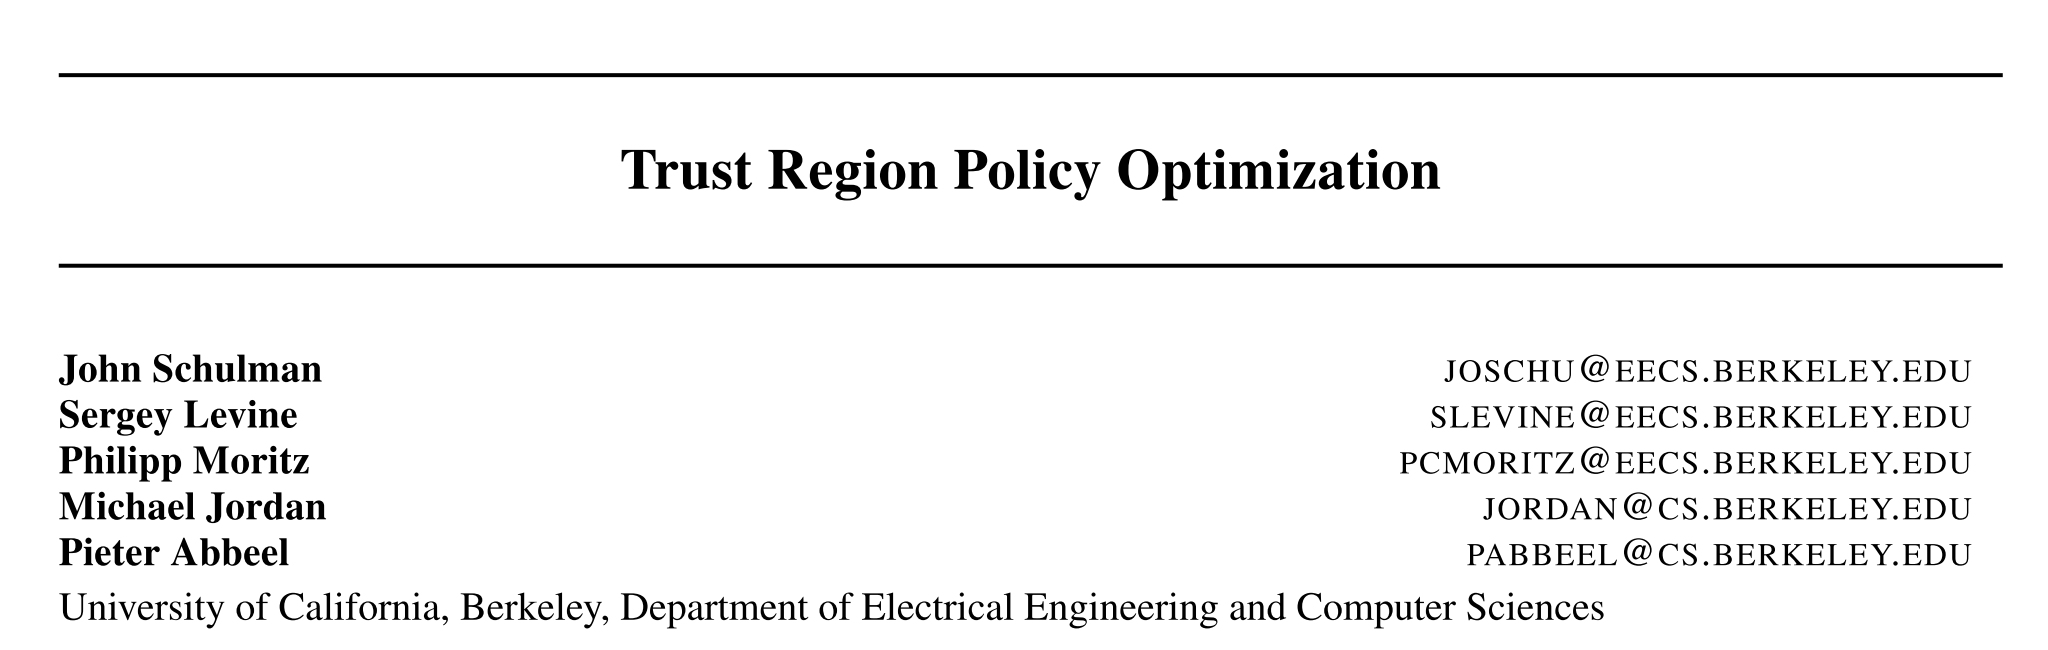
\includegraphics[width=\textwidth]{figures/paper_title.png}
\end{figure}
\begin{itemize}
    \item Kakade, Sham M. "A natural policy gradient." Advances in neural information processing systems 14 (2001). (910 citations)
    \item \textbf{Schulman, John, et al. "Trust region policy optimization." International conference on machine learning. PMLR, 2015. (3826 citations)}
    \item Schulman, J., Wolski, F., Dhariwal, P., Radford, A., \& Klimov, O. (2017). Proximal policy optimization algorithms. arXiv preprint arXiv:1707.06347. (5066 citaions)
\end{itemize}

\end{frame}

\begin{frame}
    \frametitle{Notation}
    \begin{itemize}
        \item $P: \mathcal{S} \times \mathcal{A} \times \mathcal{S} \rightarrow \mathbb{R}$ is the transition probability distribution.
        \item $r: \mathcal{S} \rightarrow \mathbb{R}$ is the reward function.
        \item $\rho_0: \mathcal{S} \rightarrow \mathbb{R}$ is the distribution of the initial state $s_0$.
        \item $\eta(\pi) = \mathbb{E}_{s_0, a_0, \ldots } \big[ \sum^{\infty}_{t=1} \gamma^{t} r(s_t) \big]$ is the expected discounted reward, where
            \[
                s_0 \sim  \rho_0(s_0), a_t \sim \pi(a_t|s_t), s_{t+1} \sim P(s_{t+1}| s_t, a_t).
            \] 
        \item $Q_\pi(s_t, a_t) = \mathbb{E}_{s_{t+1}, a_{t+1}, \ldots } \big[ \sum^{\infty}_{\ell=0} \gamma^{\ell} r(s_{t+1})\big]$
        \item $V_\pi(s_t) = \mathbb{E}_{a_t, s_{t+1}, \ldots } \big[ \sum^{\infty}_{\ell=0} \gamma^{\ell} r(s_{t+1})\big]$
        \item $A_\pi(s, a) = Q_\pi(s, a) - V_\pi(s)$ is the advantage function.
    \end{itemize}
\end{frame}

\begin{frame}
    \frametitle{Starting Point}
    \begin{itemize}
        % \item Off-policy prediction/control is based on important sampling
        %     \[
        %         V(s) = \dfrac{1}{\abs{\mathcal{T}(s)}} \sum_{t \in \mathcal{T}(s)} \left( \prod_{k=t}^{T-1} \dfrac{\pi(A_k| S_k)}{b(A_k|S_k)} \right) G_t
        %     \] 
        \item Kakade \& Langford (2002) showed a relation between any policy $\pi$ and  $\widetilde{\pi}$. 
            \begin{equation}
                \label{eq:starting_point}
        \eta(\widetilde{\pi}) = \eta(\pi) + \mathbb{E}_{s_0, a_0, \ldots  \sim \widetilde{\pi}} \left[ \sum^{\infty}_{t=0} \gamma^{t} A_\pi(s_t, a_t) \right]
            \end{equation} 
    \begin{proof}
    Let $\tau \sim \widetilde{\pi}$ be a  trajectory sampled using $\widetilde{\pi}$.
        \begin{align*}
            &\mathbb{E}_{\tau | \widetilde{\pi}} \left[ \sum^{\infty}_{t=0} \gamma^{t} A_\pi(s_t, a_t) \right] \\
            &= \mathbb{E}_{\tau | \widetilde{\pi}} \left[ \sum^{\infty}_{t=0} \gamma^{t} (r(s_t)+ \gamma V_{\pi}(s_{t+1}) - V_\pi(s_t)) \right] \\
            &= \mathbb{E}_{\tau | \widetilde{\pi}} \left[r(s_0) + {\blue \gamma V_\pi(s_1)} - V_\pi(s_0) + \gamma (r(s_1)+ {\red \gamma V_\pi(s_2)} - {\blue V_\pi(s_1)}) + \gamma^2 (.) + \ldots \right] \\
            &= \mathbb{E}_{\tau | \widetilde{\pi}} \left[ -V_\pi(s_0) + \sum^{\infty}_{t=0} \gamma^{t} r(s_t) \right]
            = - \mathbb{E}_{s_0} \left[ V_\pi(s_0) \right] + \mathbb{E}_{\tau | \widetilde{\pi}} \gamma^{t} r(s_t) \\
            &= -\eta_{\pi} + \eta_{\widetilde{\pi}}
        \end{align*}
    \end{proof}
    \end{itemize}
\end{frame}

\begin{frame}
    \begin{itemize}
        \item Define $\rho_\pi$ is the discounted visitation frequencies, $\rho_\pi = \sum^{\infty}_{t=0} \gamma^{t} P(s_t = s)$. Note that $s_0 \sim \rho_0$, the others depend on $\pi$ and the environment.
        \item Rewrite \eqref{eq:starting_point}
        \begin{align*}
            \eta(\widetilde{\pi}) 
            &= \eta(\pi) + \mathbb{E}_{s_0, a_0, \ldots  \sim \widetilde{\pi}} \left[ \sum^{\infty}_{t=0} \gamma^{t} A_\pi(s_t, a_t) \right] \\
            &= \eta(\pi) + \sum^{\infty}_{t=0} \sum_{s} P(s_t= s| \widetilde{\pi}) \sum_{a} \widetilde{\pi}(a|s) \gamma^{t} A_\pi(s_t, a_t)  \\
            &= \eta(\pi) +  \sum_{s} \sum^{\infty}_{t=0} \gamma^{t}  P(s_t= s| \widetilde{\pi}) \sum_{a} \widetilde{\pi}(a|s) A_\pi(s_t, a_t)  \\
            &= \eta(\pi) +  \sum_{s} \rho_{\widetilde{\pi}(s)} {\blue \sum_{a} \widetilde{\pi}(a|s) A_\pi(s_t, a_t)}
        \end{align*} 
    \item If the blue term is nonnegative at every state, then $\widetilde{\pi}$ is better or equal $\pi$
    \item In deterministics setting, it reduces to policy improvement, i.e., $\widetilde{\pi}(s)  = \argmax_a A_{\pi}(s, a)$
    \item Maximizing the RHS respect to paremeters of $\widetilde{\pi}$ would result the best policy
    \end{itemize}
\end{frame}


\begin{frame}
    \frametitle{The first approximation}
\begin{itemize}
    \item Recall 
        \[ \eta(\widetilde{\pi}) = \eta(\pi) +  \sum_{s} \rho_{{\blue \widetilde{\pi}}}(s) { \sum_{a} \widetilde{\pi}(a|s) A_\pi(s_t, a_t)} \]
    \item Define 
        \[
            L_\pi(\widetilde{\pi}) \coloneqq \eta(\pi) + \sum_{s} \rho_{{\blue \pi} } (s)\sum_{a} \widetilde{\pi}(a|s) A_\pi (s_t, a_t)
        \] 
        then $L_\pi(\widetilde{\pi}) \approx \eta(\widetilde{\pi})$ locally in a sense that
        \[
            L_{\pi_{\theta_0}}(\pi_{\theta_0}) = \eta (\pi_{\theta_0}), \quad \text{and } \nabla_{\theta} L_{\pi_{\theta_0}}(\pi_{\theta})  \mid_{\theta = \theta_0} \; = \; \nabla_{\theta} \eta(\pi_{\theta}) \mid_{\theta = \theta_0}
        \] 
    \item The first equality holds since $ \underbrace{\sum_{s} \rho_{\pi}(s) \sum_{a} \pi(a|s)}_{ \mathbb{E}} (Q_\pi(a, s) - V_\pi(s)) = 0$
    % \item The second equality holds by taking derivative of both equations, and the result is 
    %     \[
    %         \sum_{s}  \rho_{\pi_{\theta_0}} (s) \sum_{a} A_{\pi_{\theta_0}}(s_t, a_t) \nabla \pi_{\theta_0} (a|s)
    %     \] 
    \item An improvement is guaranteed if using the following updating rule 
        \[
            \pi_{\rm new} (a|s) = (1 - \alpha) \pi_{\rm old} (a|s) + \alpha \pi'(a|s),
        \] 
        where $\pi' = \argmax_{\pi} L_{\pi_{\rm old}}(\pi)$ and it is bounded by
        \[
            \eta(\pi_{\rm new}) \geq L_{\pi_{\rm old}} (\pi_{\rm new}) - \dfrac{2\epsilon \gamma }{(1- \gamma)^2} \alpha^2
        \] 
    \item Maximizing $L_{\pi_{\rm old}}(\pi_\theta)$ respect to $\theta$ is guaranteed to improve over $\pi_{\rm old}$
\end{itemize}
\end{frame}


\begin{frame}
    \frametitle{New lower bound}

\begin{itemize}
    \item Define $D_{\rm TV}(p || q) = \dfrac{1}{2} \sum_{i=1} \abs{p_i - q_i}$ (called total variation divergence), and
\item $D_{\rm TV}^{\max}(\pi, \widetilde{\pi}) = \max_s D_{\rm TV}(\pi( a| s ), \widetilde{\pi}(a|s))$
\end{itemize}

    \begin{theorem}
        Let $\alpha = D^{\rm max}_{\rm TV} (\pi_{\rm old}, \pi_{\rm new})$. Then the following bound holds
        \[
            \eta(\pi_{\rm new}) \geq L_{\pi_{\rm old}}(\pi_{\rm new}) - \dfrac{4\epsilon \gamma}{(1-\gamma)^2} \alpha^2, 
        \] 
        where $\epsilon = \max_{a,s} \abs{A_\pi(s, a)}$
    \end{theorem}

    \textit{The improvement is guaranteed to general stochastic policy.}
\end{frame}

\begin{frame}
    \frametitle{Algorithm}
    \begin{itemize}
    \item Define $D_{\rm KL}^{\max} (\pi, \widetilde{\pi}) = \max_s D_{\rm KL} (\pi(a|s), \widetilde{\pi}(a|s))$
    \item Since $D_{\rm TV}(p || q)^2 \leq D_{\rm KL}(p || q)$
            \begin{equation}
                \label{eq:policy_improvement}
                \eta(\pi_{\rm new}) \geq L_{\pi_{\rm old}}(\pi_{\rm new}) - \dfrac{4\epsilon \gamma}{(1-\gamma)^2} D_{\rm KL}^{\max}(\pi_{\rm old}, \pi_{\rm new})
            \end{equation} 
    \end{itemize}

    \begin{columns}
        \begin{column}{0.4\textwidth}
        \begin{figure}
            \centering
            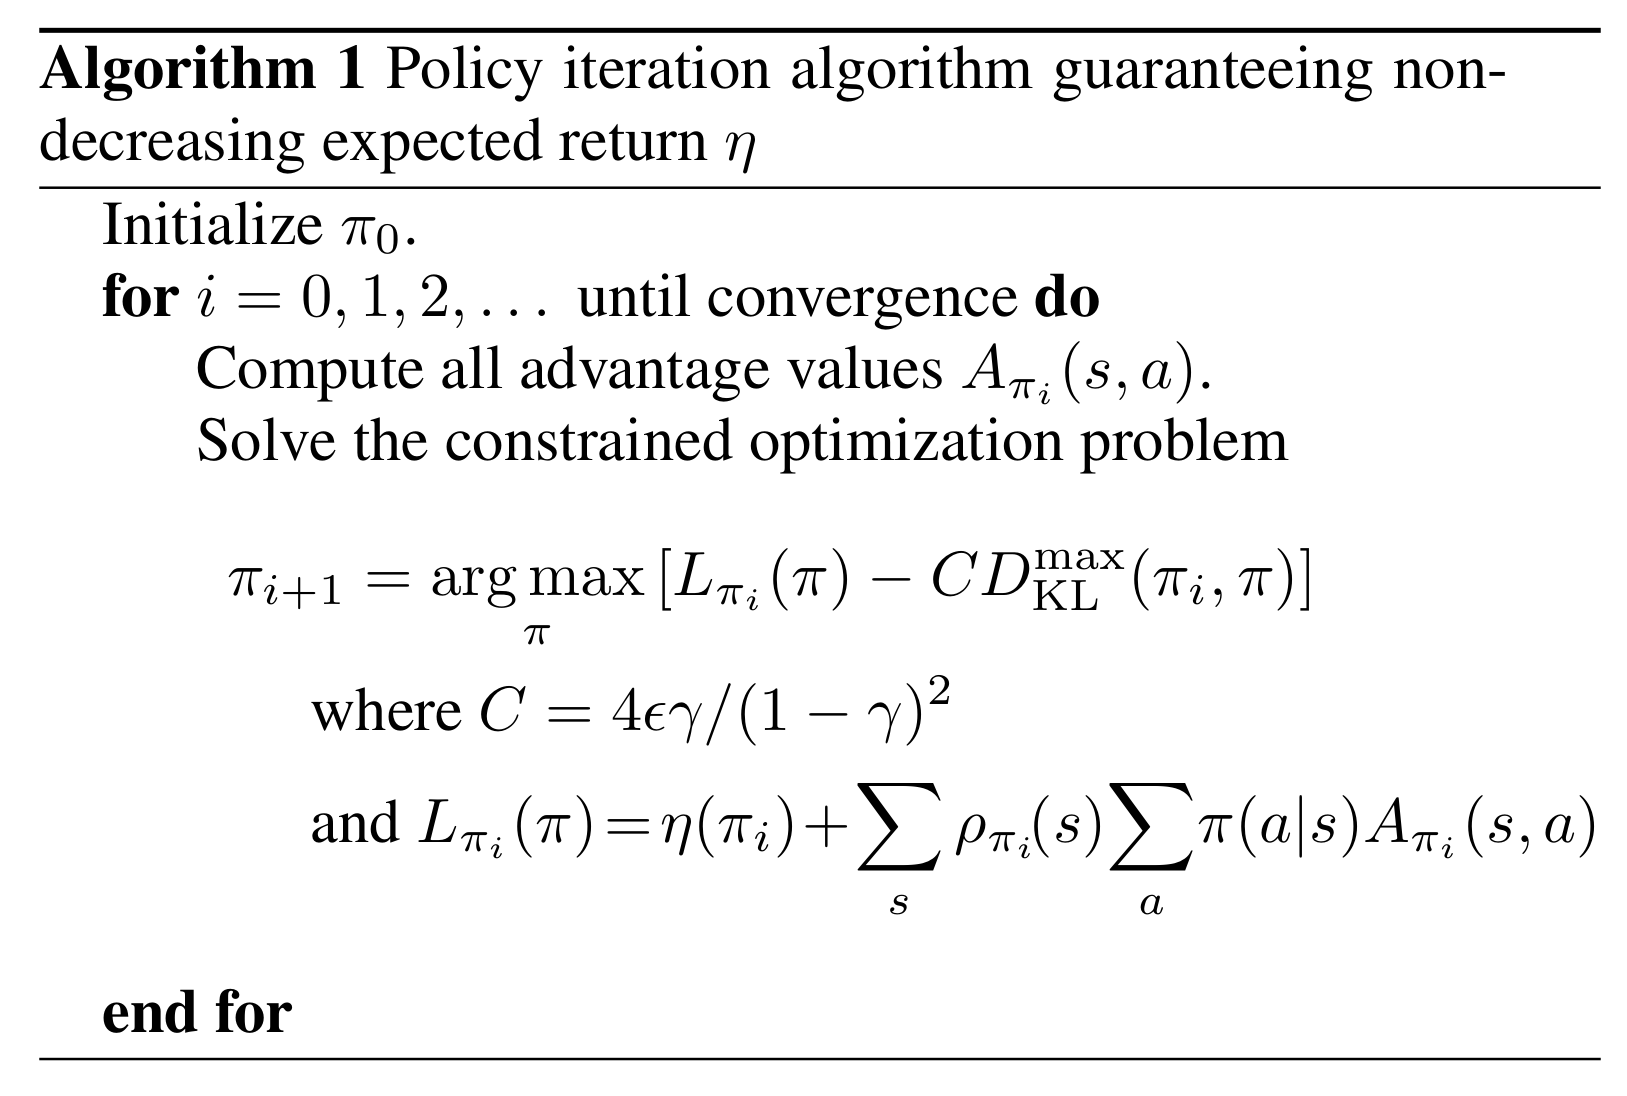
\includegraphics[width=\textwidth]{figures/alg1.png}
        \end{figure}
        \end{column}
        \begin{column}{0.55\textwidth}
            Policy improvement guarantee: 
            \begin{itemize}
                \item Let $M_i(\pi) = L_{\pi_i}(\pi) - C D_{\rm KL}^{\max}(\pi_i, \pi) $
                    \begin{align*}
                        \eta(\pi_{i+1}) 
                        &\geq M_i(\pi_{i+1}) \quad \text{(by \ref{eq:policy_improvement})} \\
                        &\geq M_i(\pi_i) \quad \text{(by updating rule)} \\
                        &= \eta(\pi_i)
                    \end{align*}
            \end{itemize}
        \end{column}
    \end{columns}
    \begin{itemize}
        \item The algorithm design is a type of minorization-minimization, where $M_i$ is the surrogate function
        \item It is slow if $C$ large
        \item Optimization problem:
            \begin{align*}
                &\max_{\theta} L_{\theta_{old}} (\theta)  \\
                &\text{subject to } D_{\rm KL}^{\max} (\theta_{\rm old}, \theta) \leq \delta
            \end{align*} 
    \end{itemize}

\end{frame}

\begin{frame}
    \frametitle{The second approximation}
    Let $\overline{D}_{\rm KL}^{\rho} = \mathbb{E}_{s \sim \rho} [D_{\rm KL}] (\pi_{\theta_1} (\cdot|s)| \pi_{\theta_2}(\cdot|s))$
    \begin{itemize}
        \item Relax constrain to $ \overline{D}^{\rho_{\rm old}}_{\rm KL} (\theta_{\rm old}, \theta) \leq \delta $ 
        \item Rewrite the objective function in expectation form
            \begin{align*}
                &\argmax_{\theta} \sum_{s} \rho_{\theta_{\rm old}}(s)\sum_{a} \pi_{\theta}(a|s) A_{\theta_{\rm old}}(s, a)  \\
                &= \argmax_{\theta} \left(  \sum_{s} \rho_{\theta_{\rm old}}(s) \sum_{a} \pi_{\theta}(a|s) Q_{\theta_{\rm old}}(s,a) - \sum_{s} \rho_{\theta_{\rm old}(s)} \sum_{a} \pi_{\theta}(a|s) V_{\theta_{\rm old}}(s) \right)\\
                &= \argmax_{\theta} \sum_{s} \rho_{\theta_{\rm old}}(s) \mathbb{E}_{a \sim q} \dfrac{\pi_{\theta}(a|s)}{q(a|s)}Q_{\theta_{\rm old}} \\
                &= \argmax_{\theta} \; \mathbb{E}_{s \sim \rho_{\rm old}, a \sim q} \dfrac{\pi_{\theta}(a|s)}{q(a|s)}Q_{\theta_{\rm old}} \\
            \end{align*}
        \item Final optimization problem
            \begin{align*}
                &\min_{\theta} \; \mathbb{E}_{s \sim \rho_{\rm old}, a \sim q} \left[  \dfrac{\pi_{\theta}(a|s)}{q(a|s)}Q_{\theta_{\rm old}}\right] \\
                &\text{subject to } \mathbb{E}_{s \sim \rho_{\theta_{\rm old}}} [D_{\rm KL}(\pi_{\rm old}( \cdot| s ) || \pi_{\rm new}( \cdot| s ))] \leq \delta
            \end{align*}
            where $q$ is behaviour policy,  $q = \pi_{\theta_{\rm old}}$
    \end{itemize}
\end{frame}

\begin{frame}
    \frametitle{Pratical algorithm - The third approximation}
    \begin{equation}
        \label{eq:final_opt}
    \begin{aligned}
        &\min_{\theta} \; \mathbb{E}_{s \sim \rho_{\rm old}, a \sim q} \left[  \dfrac{\pi_{\theta}(a|s)}{q(a|s)}Q_{\theta_{\rm old}}\right] \\
        &\text{subject to } \mathbb{E}_{s \sim \rho_{\theta_{\rm old}}} [D_{\rm KL}(\pi_{\rm old}( \cdot| s ) || \pi_{\rm new}( \cdot| s ))] \leq \delta
    \end{aligned}
    \end{equation}
    \begin{columns}
        \begin{column}{0.7\textwidth}
    Repeat the following steps:
    \begin{itemize}
        \item Use Monte Carlo simulation to collect trajectories.
            \begin{itemize}
                \item Single path: generate 1 episode, then move to step 2
                \item Vine: generate a number of trajectories, then choose a subset of states and samples actions from these state to generate new branching trajectories.
            \end{itemize}
        \item Construct the estimated objective and constraint of Problem \eqref{eq:final_opt}
        \item Approximately solve this optimization problem using conjugate gradient algorithm followed by a line search.
    \end{itemize}
        \end{column}
        
        \begin{column}{0.3\textwidth}
            \begin{figure}
                \centering
                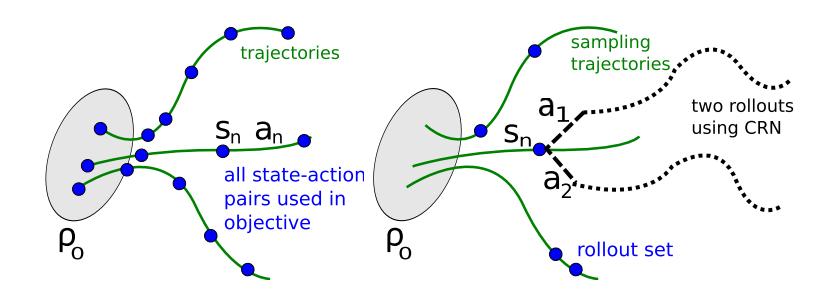
\includegraphics[width=1.2\textwidth]{figures/mc.png}
            \end{figure}
        \end{column}
    \end{columns}
\end{frame}


\begin{frame}
    \frametitle{Experiment result}
    \begin{figure}
        \centering
        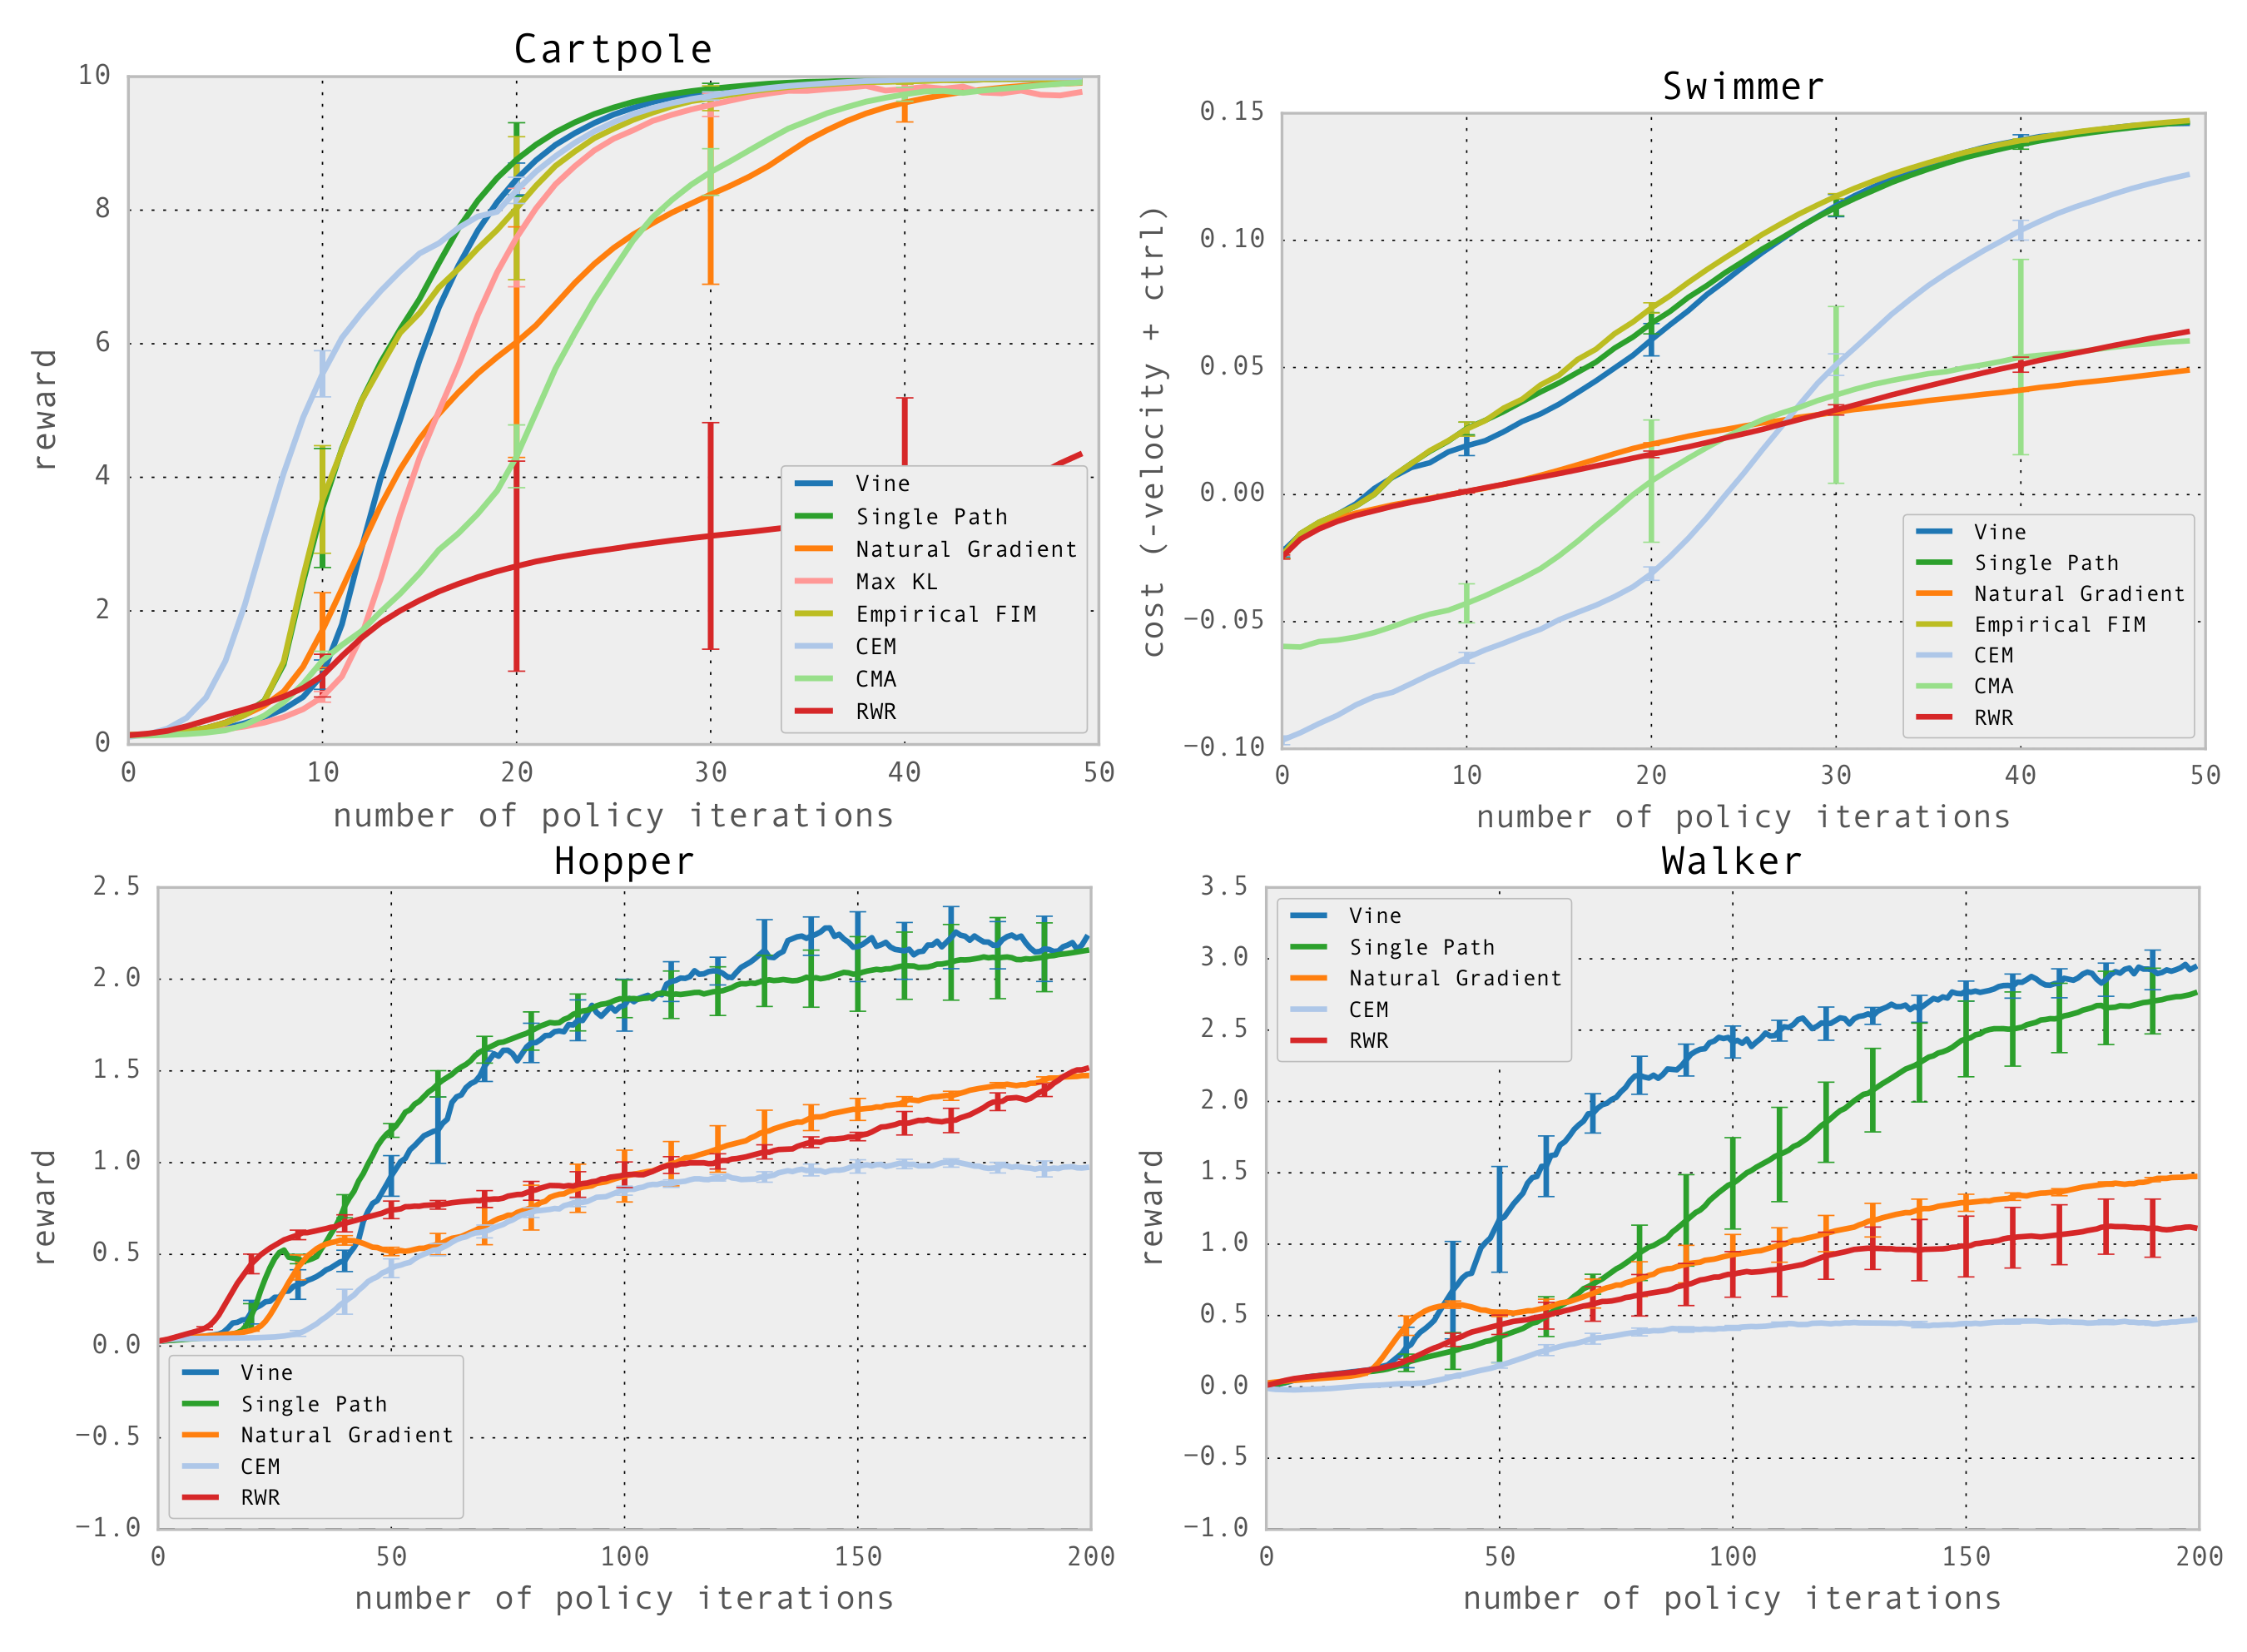
\includegraphics[width=0.7\textwidth]{figures/result1.png}
    \end{figure}

\end{frame}

\begin{frame}
    \frametitle{Experiment result}
    \begin{figure}
        \centering
        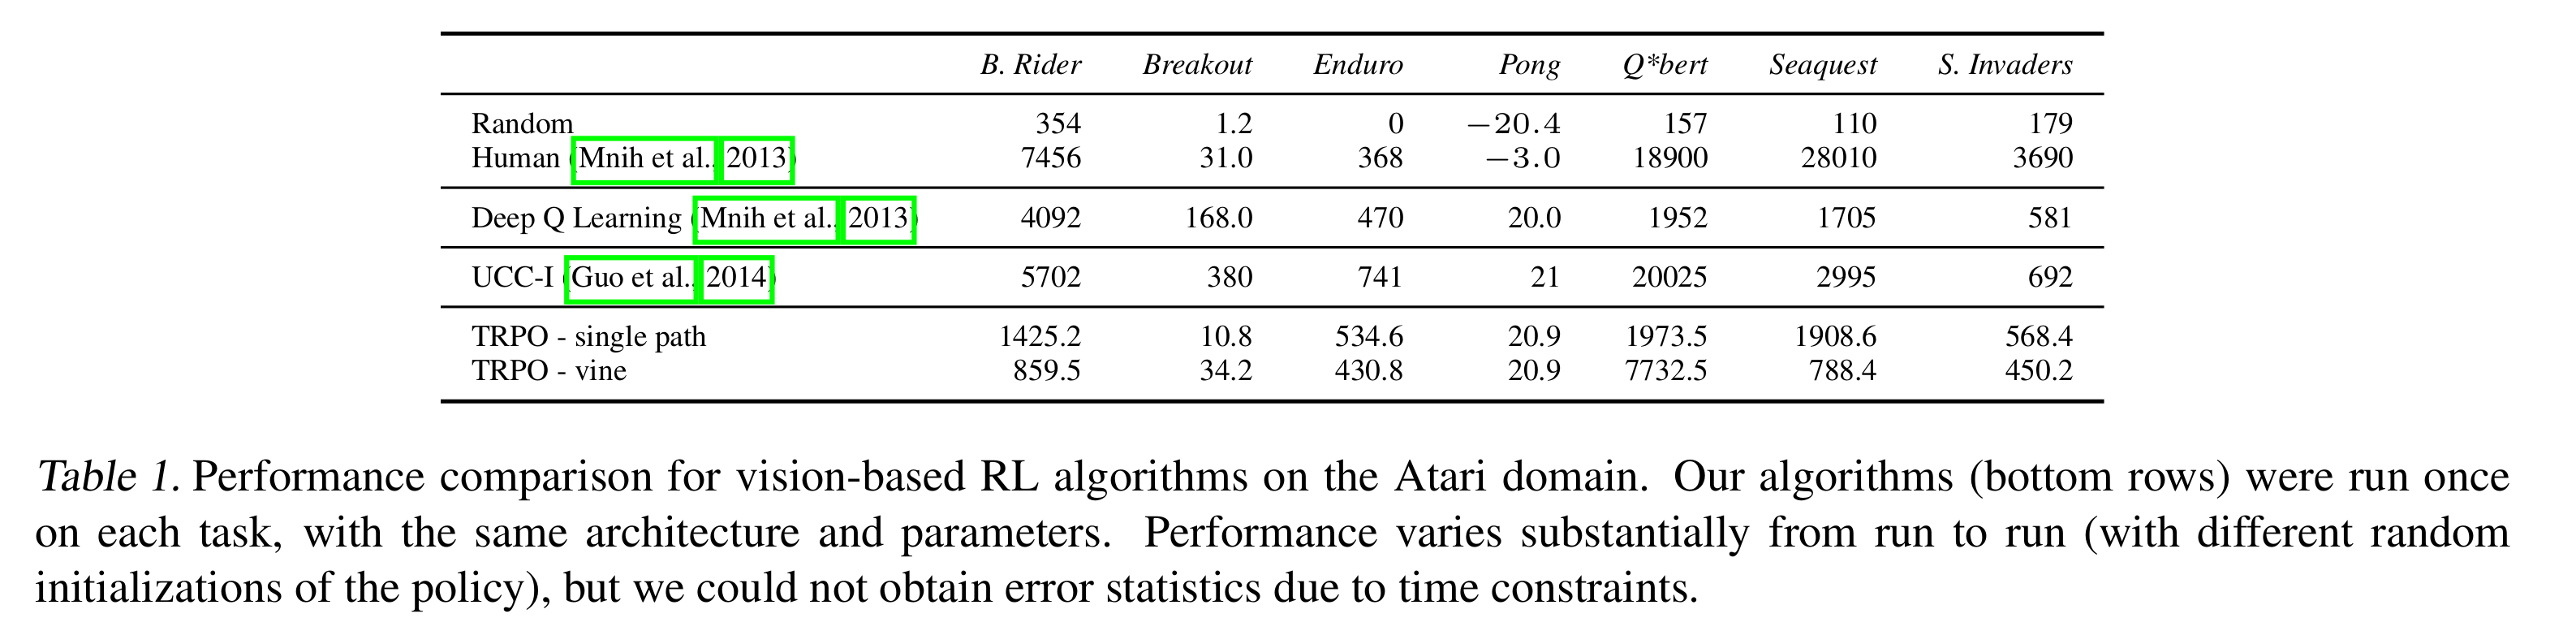
\includegraphics[width=\textwidth]{figures/result2.png}
    \end{figure}
\end{frame}

\begin{frame}
    \frametitle{Conclusion}
    \begin{itemize}
        \item Theorem 1 justifies for the surrogate objective function.
        \item Proposing using hard constraint instead of using penalty objective.
        \item Single path or vine using MC for estimating the minimization problem.
        \item Using conjugate gradient method for search direction, and line search to ensure the current step satisfies constraint.
    \end{itemize}
\end{frame}



\begin{frame}
    \frametitle{Optimization method}
        \begin{align*}
            &\max_{\theta} L_{\theta_{old}} (\theta)  \\
            &\text{subject to } \overline{D}_{\rm KL} (\theta_{\rm old}, \theta) \leq \delta
        \end{align*} 

    Step 1: find the optimal direction to update
    \begin{itemize}
        \item The fisher information matrix is defined as $ \bm{F} = \mathbb{E}_{x \sim p(x; \theta)} [\nabla \log p(x; \theta) \nabla \log p(x; \theta)^T ]$
        \item Fact: $ \bm{F} = - \bm{H}_{\theta} [\log \nabla p(x; \theta)] $
        \item A derived fact: $\bm{F} = \bm{H}_{D_{\rm KL}}$ 
        \item A derived approximation:
            $ D_{\rm KL}(p_{\theta} || p_{\theta'}) \approx \dfrac{1}{2} (\theta' - \theta)^T \bm{F} (\theta' - \theta) $

    \end{itemize}
    Then we can dirive the optimal direction by
    \begin{itemize}
        \item Linear approximation of the objective:
\[
    L_{\theta_{\text{old}}}(\theta) \approx L_{\theta_{\text{old}}} + \nabla_{\theta} L_{\theta_{\text{old}}}(\theta)\mid_{\theta = \theta_{\text{old}}} [ \theta - \theta_{\text{old}} ] 
\] 
    \item Quadratic approximation of the constrain:
\[
    D_{\rm KL}(\theta_{\text{old}}, \theta) \approx \dfrac{\lambda}{2} (\theta - \theta_{\text{old}})^T \bm{F} (\theta - \theta_{\text{old}}),
\] where $\bm{F}$ is Fisher information matrix.
\item Lagrangian form 
\[
    f(\theta) := L_{\theta_{\text{old}}} + \nabla_{\theta} L_{\theta_{\text{old}}}(\theta)\mid_{\theta = \theta_{\text{old}}} [ \theta - \theta_{\text{old}} ] 
    + \dfrac{\lambda}{2} (\theta - \theta_{\text{old}})^T \bm{F} (\theta - \theta_{\text{old}})
\] 
    \end{itemize}

\end{frame}

\begin{frame}
    \frametitle{Find optimal direction}
    \begin{itemize}
        \item To find optimal $f^{*}$, we can find $\theta^{*}$ such as $\nabla f(\theta^{*}) = 0$,
                \[
                    0 = \nabla_{\theta} L_{\text{old}}(\theta) \mid_{\theta = \theta_{\text{old}}} + \lambda \bm{F}(\theta^{*} - \theta_{\text{old}})  \Leftrightarrow \theta^{*} = \theta_{\text{old}} - \lambda \bm{F}^{-1} \nabla_{\theta} L_{\theta_{\text{old}}}(\theta) \mid_{\theta = \theta_{\text{old}}}
                \] 
            \item Therefore, the optimal direction is $\bm{y} = \bm{F}^{-1} \nabla_{\theta} L_{\theta_{\text{old}}}(\theta) |_{\theta = \theta_{\text{old}}}$
            \item Conjugate gradient can be used to solve $\bm{F}\bm{y} = \nabla_{\theta} L_{\theta_{\text{old}}}(\theta) \mid_{\theta = \theta_{\text{old}}}$
    \end{itemize}
\end{frame}

\begin{frame}
    \frametitle{Connection to other methods}
\begin{itemize}
    \item Standard policy gradient 
        \begin{align*}
            &\max_{\theta} \; \left[ \nabla_{\theta}L_{\theta_{\text{old}}}(\theta) \mid_{\theta=\theta_{\text{old}}} \cdot (\theta - \theta_{\text{old}}) \right] \\
            &\text{subject to } \dfrac{1}{2} \norm{\theta - \theta_{\text{old}}}^2 \leq \delta
        \end{align*} 
    \item Natural policy gradient  (Kakade, 2002)
        \begin{align*}
            &\max_{\theta} \; \left[ \nabla_{\theta}L_{\theta_{\text{old}}}(\theta) \mid_{\theta=\theta_{\text{old}}} \cdot (\theta - \theta_{\text{old}}) \right] \\
            &\text{subject to } \dfrac{1}{2}(\theta_{\text{old}} - \theta)^T \bm{F} (\theta_{\text{old}} - \theta) \leq \delta
        \end{align*} 
\end{itemize}
\end{frame}

\begin{frame}
    \frametitle{Proximal policy optimization}
    ``Proximal policy optimization algorithms" (PPO) improved upon this by using only first-order derivative.
    \begin{itemize}
        \item Recall the objective in TRPO is
            \[
                \mathbb{E} \left[ \dfrac{\pi_{\theta}(a|s)}{\pi_{\theta_{\text{old}}}(a|s)} Q_{\theta_{\text{old}}} \right] = \mathbb{E}[r(\theta) Q_{\theta_{\text{old}}}]
            \] 
        \item In PPO, the objective is
            \[
                \mathbb{E} \left[  \min(  r(\theta) Q_{\theta_{\text{old}}} , \text{clip}(r(\theta), 1-\epsilon, 1+\epsilon)Q_{\theta_{\text{old}}}) \right]
            \] 
    \end{itemize}
\end{frame}

\begin{frame}
    \frametitle{PPO experiment result}
    \begin{figure}
       \centering
       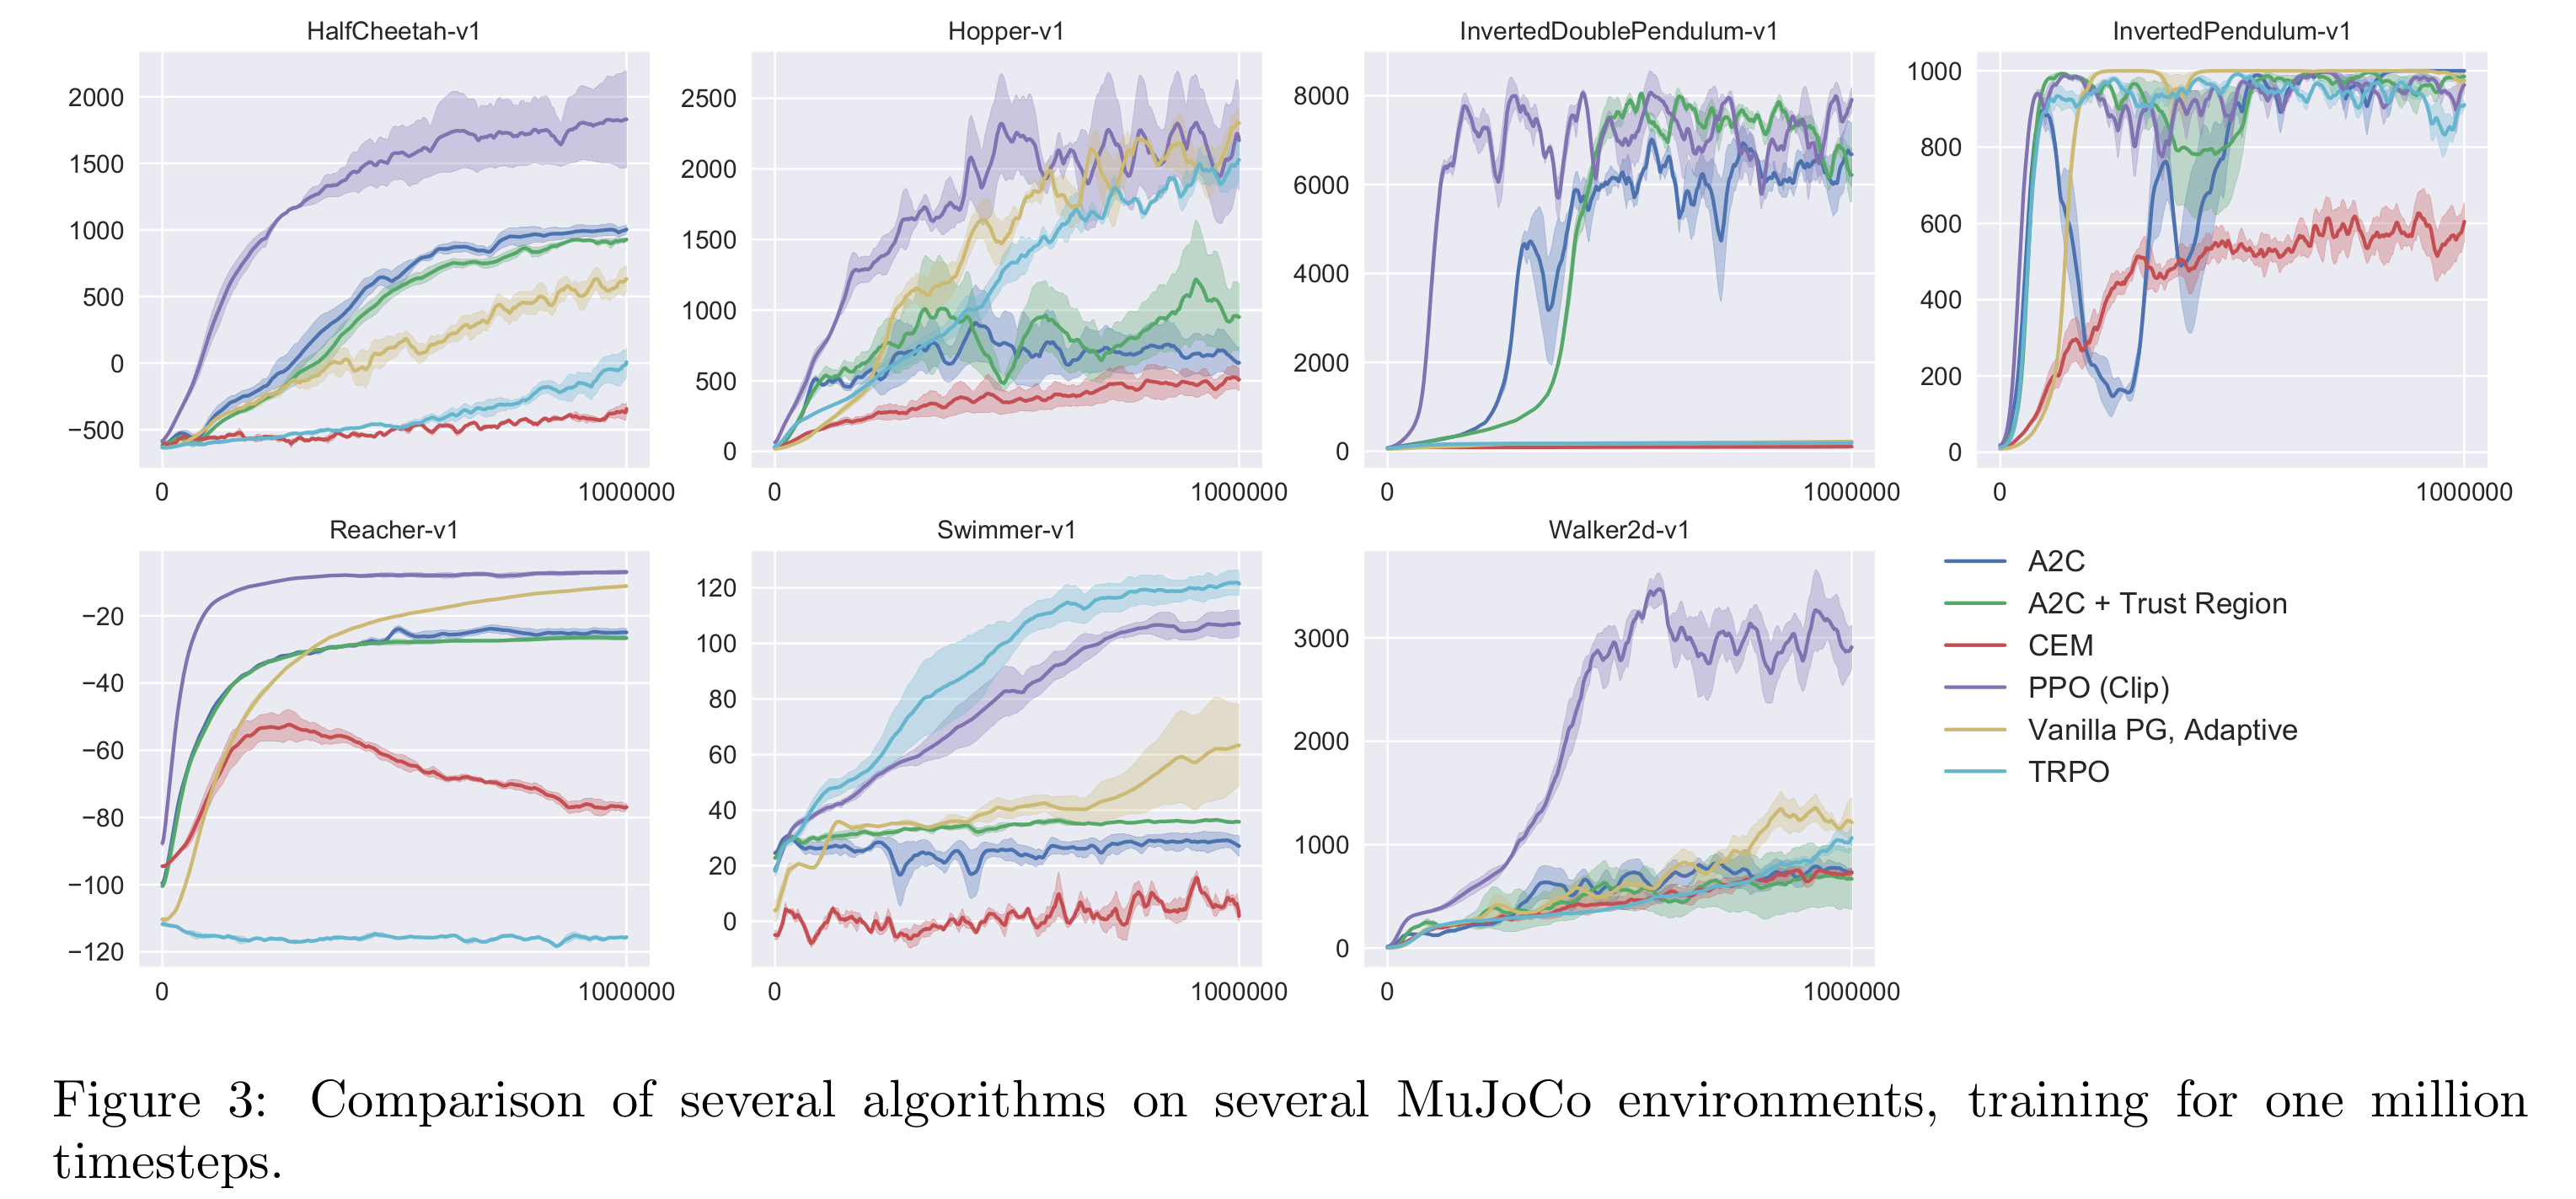
\includegraphics[width=0.9\textwidth]{figures/ppo.png}
   \end{figure}    
\end{frame}
\end{document}

